\hthree{LXC VS. Docker}

\hfour{Architektur}

Im Kern ähnelt sich die Systemarchitektur von LXC jener von Docker, da die wichtigsten verwendeten Funktionen des Linux-Kernel "cgroups" und "namespaces" sind. "Cgroups" sind hierbei für die Aufteilung von CPU, Speicher und vielem mehr im System zuständig. "Namespaces" erlauben das Erstellen von mehreren virtuellen Instanzen des Kernels. Es kann daher gesagt werden, dass sich LXC und Docker im Bereich des Systemkernels sehr ident sind. \cite{LxcVsDocker}

Im Bereich der Engine, welche zwischen Anwendung und Kernel liegt, setzt LXC auf das Framework "liblxc". Docker implementierte jedoch ihre eigene Engine, welche den Namen "libcontainer" trug. Diese wurde jedoch im Laufe der Jahre durch mehrere dazwischenliegende Abstraktionsschichten ergänzt. \cite{LxcVsDocker}

Die gesamte Architektur von Docker ist jedoch nicht ganz so trivial. Der grobe Ablauf beim Zugriff auf Daten sieht wie folgt aus:

Zu Beginn greift der Client auf den "Docker Deamon" zu, welcher auf einem "Docker\_Host" liegt. Dieser stellt die Hauptbenutzeroberfläche zur Verfügung. Der "Docker Deamon" greift nun auf ein Image im Host zu, welches schreibgeschützt ist. Es kann jedoch Images mehrere Container geben, auf welchen dann die gewünschten Änderungen des Clients durchgeführt werden. \cite{LxcVsDocker}

\begin{figure}[H]
    \centering
    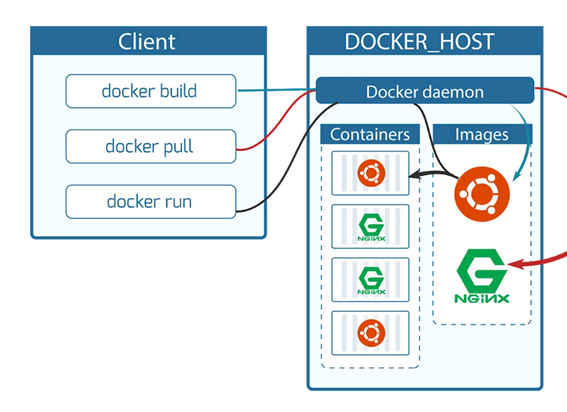
\includegraphics{media/DockerAndContainering/DockerArchitektur.png}
    \caption{Docker Architektur \cite{LxcVsDocker}}
\end{figure}

\hfour{Speicherverwaltung}

Bei LXC ist die Speicherverwaltung recht einfach gemacht worden. Sofern keine anderen Optionen gewählt wurden, legt LXC die Daten unter dem Linux Pfad: "/var\-/lib\-/lxc\-/[container-name]/rootfs" ab. Die Einbindung von Datenbanken oder eines NAS-Systems (Network Attached Storage) funktioniert ohne große Probleme, da alles über das "rootfs" des jeweiligen Containernamen abgewickelt wird. \cite{LxcVsDocker}

Bei Docker funktioniert das Ganze ein bisschen anders. Hierbei wird das Image normal in seiner Gesamtheit abgelegt. Das Image verweist jedoch auf eine Vielzahl von Speicherebenen, welche eben einem Image eindeutig zugeordnet sind. Diese Ebenen werden beim Erzeugen übereinandergestapelt. Dieser Speicherstapel des Images ist dann die Basis des sogenannten "Container-Root-Dateisystems". Für das Übereinanderstapeln und das generelle Verwalten der Speicherebenen ist der Treiber des "Docker Storage" zuständig. Außerdem verwaltet dieser Treiber auch das gemeinsame Verwenden von Speicherebenen zwischen Containern. Ein Vorteil, welcher sich einerseits aus diesem Verwaltungsmechanismus und andererseits aus der gegenseitigen Nutzbarkeit ergibt, ist auf der einen Seite das vereinfachte Erstellen, Verschieben oder Kopieren des gesamten Images und auf der anderen Seite spart die gemeinsame Nutzung Speicherplatz auf dem System. \cite{LxcVsDocker}

Sobald die User*innen einen neuen Container erzeugen, passiert Folgendes: Es wird auf das angegebene Image zugegriffen, welches jedoch schreibgeschützt ist. Deshalb bekommt jeder einzelne Container eines Images eine eigene Speicherebene in diesem Gesamtimage. So greift jeder Container nur auf seinen Speicherstand zu und man kann von einem Image auch mehrere unterschiedliche Speicherstände haben. \cite{LxcVsDocker}

\begin{figure}[H]
    \centering
    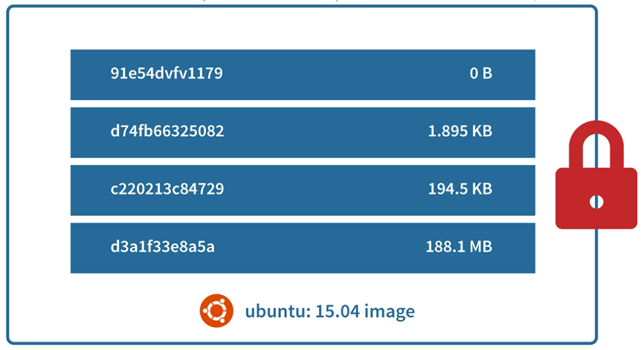
\includegraphics{media/DockerAndContainering/Speicherebenen.png}
    \caption{Speicherebenen in Docker \cite{LxcVsDocker}}
\end{figure}

Docker arbeitet beim Schreiben oder Ändern von Images oder Containern mit der sogenannten "Copy-on-Write"(CoW)-Technologie. Dies ist ein Optimierungsverfahren, welches für das Schreiben zwischen zwei Prozessen auf unixartigen Systemen eingesetzt wird. Die Grundidee dahinter ist, dass eine Kopie einer Datei erst real angelegt wird, wenn sie sich von der "Mutterdatei" unterscheidet. Für Docker bedeutet das eine Optimierung von der Nutzung des Plattenplatzes und bessere Startzeiten für die jeweiligen Container. \cite{LxcVsDocker}
